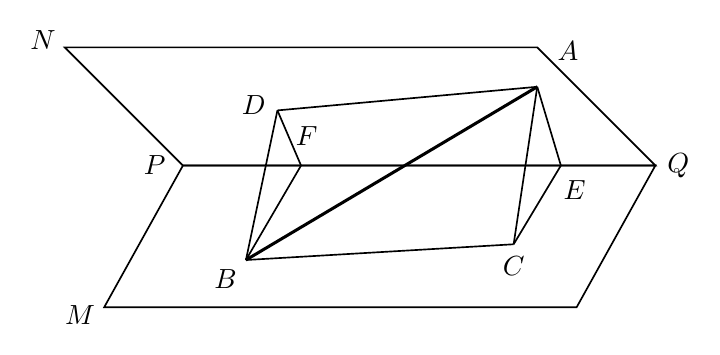
\begin{tikzpicture}[x=1cm,y=1cm,line width=0.6pt]
\tikzset{ptlabel/.style={font=\normalsize,fill=white,inner sep=1pt}}
\coordinate (P) at (-3,0);
\coordinate (Q) at (3,0);
\coordinate (A) at (1.5,1.0);
\coordinate (E) at (1.8,0);
\coordinate (C) at (1.2,-1.0);
\coordinate (F) at (-1.5,0);
\coordinate (D) at (-1.8,0.7);
\coordinate (B) at (-2.2,-1.2);
% plane outlines
\draw[draw=black] (P) -- (-4.5,1.5) -- (1.5,1.5) -- (Q) -- cycle;
\draw[draw=black] (P) -- (-4,-1.8) -- (2,-1.8) -- (Q) -- cycle;
\draw[draw=black] (P) -- (Q);
% right triangle AEC
\draw[draw=black] (A) -- (E);
\draw[draw=black] (E) -- (C);
\draw[draw=black] (A) -- (C);
% left triangle BFD
\draw[draw=black] (B) -- (F);
\draw[draw=black] (F) -- (D);
\draw[draw=black] (B) -- (D);
% cross links and bold AB
\draw[draw=black] (B) -- (C);
\draw[draw=black] (D) -- (A);
\draw[draw=black,line width=1.1pt] (B) -- (A);
% labels with clearance
\node[ptlabel,anchor=east,xshift=-3pt,fill=none,xshift=-2.00bp,yshift=0.00bp] at (P) {$P$};
\node[ptlabel,anchor=west,xshift=3pt] at (Q) {$Q$};
\node[ptlabel,anchor=south west,xshift=2pt,yshift=2pt,fill=none,xshift=4.00bp,yshift=6.00bp] at (A) {$A$};
\node[ptlabel,anchor=north,yshift=-4pt,xshift=5pt] at (E) {$E$};
\node[ptlabel,anchor=north,yshift=-3pt] at (C) {$C$};
\node[ptlabel,anchor=south,yshift=4pt,fill=none,xshift=2.00bp,yshift=2.00bp] at (F) {$F$};
\node[ptlabel,anchor=east,xshift=-3pt,yshift=2pt] at (D) {$D$};
\node[ptlabel,anchor=north east,xshift=-2pt,yshift=-2pt] at (B) {$B$};
\node[ptlabel,anchor=north east,xshift=-2pt,yshift=2pt] at (-4,-1.8) {$M$};
\node[ptlabel,anchor=south east,xshift=-2pt,yshift=-2pt] at (-4.5,1.5) {$N$};
\end{tikzpicture}
